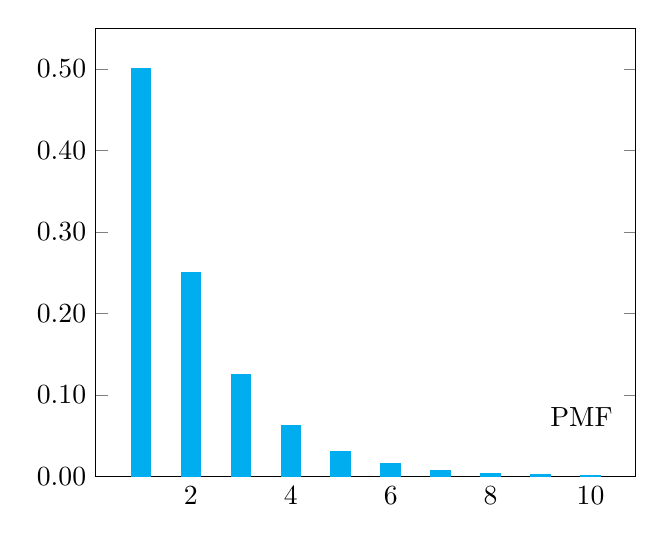
\begin{tikzpicture}
  \begin{axis}[
      ymin=0,
      ymax=0.55,
      xtick={0,2,...,10},
      ytick={0,0.1,...,0.5},
      samples at={1,...,10},
      xtick style={draw=none},
        yticklabel style={
            /pgf/number format/fixed,
            /pgf/number format/fixed zerofill,
            /pgf/number format/precision=2,
      },   
      domain=1:10,
      samples=10,
  ]
  % Define p, probability of success
  \pgfmathsetmacro{\p}{0.5}
  
  % Plot the PMF of the geometric distribution
  \addplot [
    ybar=0pt,
    bar width=7pt,
    fill=cyan,
    draw=cyan,
    mark=none,
] {(\p*(1-\p)^(x-1))};
% Add "discrete CDF" label
\node[anchor=south west] at (axis cs:9,0.05) {PMF};
  \end{axis}
\end{tikzpicture}